\section{OSI Referenzmodell}

\begin{concept}{Klassifizierung von Diensten}
    
    \begin{minipage}{0.6\linewidth}
        \textcolor{darkturquoise}{Verbindungsorientiert}
        \begin{itemize}
            \item Verbindungsaufbau nötig
            \item Informationen vom Empfänger\\ $\rightarrow$ Optionen aushandeln
            \item Reihenfolge der Daten bleibt erhalten
        \end{itemize}
    \end{minipage}
    \begin{minipage}{0.39\linewidth}
        \textcolor{darkturquoise}{Verbindungslos}
        \begin{itemize}
            \item Jederzeit\\ (send \& forget)
            \item Ziel muss nicht bereit sein
            \item einfacher umzusetzen
        \end{itemize}
    \end{minipage}

    \vspace{0.5mm}

    \begin{minipage}{0.6\linewidth}
        \textcolor{darkturquoise}{Zuverlässig}
        \begin{itemize}
            \item Kein Datenverlust
            \item Sicherung durch\\Fehler-Erkennung/-Korrektur
            \item Text-Nachrichten
        \end{itemize}
    \end{minipage}
    \begin{minipage}{0.39\linewidth}
        \textcolor{darkturquoise}{Unzuverlässig}
        \begin{itemize}
            \item Möglicher Datenverlust
            \item Keine Sicherung/ \\ Garantie
            \item $\oslash$ Flow Control etc
        \end{itemize}
    \end{minipage}

    \vspace{1mm}

    \resizebox{0.8\linewidth}{!}{
    \begin{tabular}{|l|c|c|}
        \hline & Verbindungsorientiert & Zuverlässiger Dienst \\
        \hline Ethernet & $O$ & $O$ \\
        \hline IP & 0 & 0 \\
        \hline TCP & $X$ & $\times$ \\
        \hline UDP & 0 & 0 \\
        \hline
        \end{tabular}}
\end{concept}

\centering
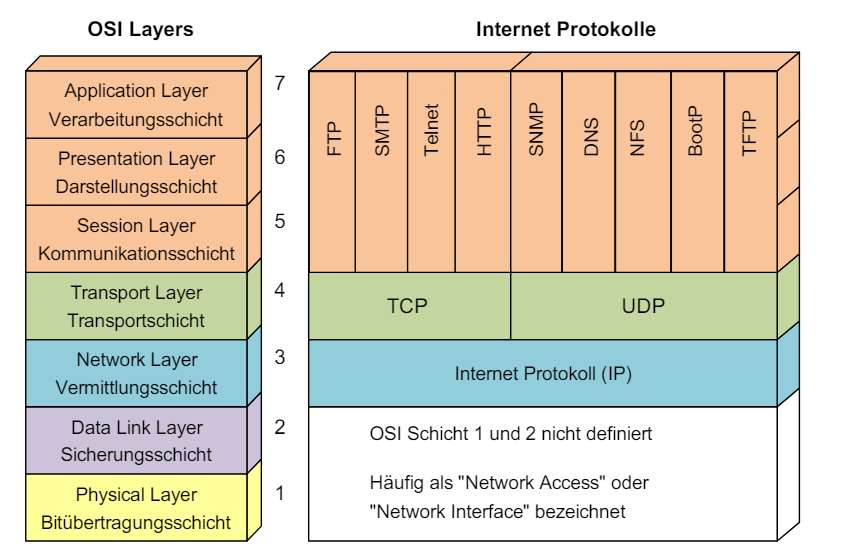
\includegraphics[width=0.8\linewidth, height=0.4\linewidth]{images/OSI_Modell.png}

\begin{KR}{Aufgaben der Schichten:} (5 und 6 nicht prüfungsrelevant)\\
    \textcolor{darkcorn}{1. Physical Layer:} ungesicherte Übertragung eines Bitstroms
    \begin{itemize}
        \item Bitübertragung, Signalisierung, Bit-Synchronisation
        \item Definiert technische Details der Übertragung: 
        Elektrische Eigenschaften, 
        Codierung, 
        Mechanische Eigenschaften
        \item Standards: USB, Ethernet, WLAN, Bluetooth, etc.
    \end{itemize}
    \textcolor{darkpurple}{2. Data Link Layer:} Realisieren einer zuverlässigen Verbindung
    \begin{itemize}
        \item Fehlererkennung und -korrektur (z.B. CRC, Hamming-Code)
        \item Framing/Frame Delineation (Präambel/SFD) 
        \item Flow-Control (Vermeidung von Überlastung) 
        \item Adressierung, Media Access Control (CSMA/CD), Timing
        \item Protokolle: Ethernet, VLAN, Spanning Tree Protocol (STP), etc.
    \end{itemize}
    \textcolor{darkblue}{3. Network Layer:} Verbindet Netze, ermöglicht Kommunikation
    \begin{itemize}
        \item Adressierung, Routing, Weiterleitung von IP-Paketen
        \item Fragmentierung, Reassembly, Kapselung und Adressauflösung (ARP), Übertragung von Fehlermeldungen (ICMP)
        \item Protokolle: IP, ICMP, ARP, etc.
    \end{itemize}
    \textcolor{darkgreen}{4. Transport Layer:} Schnittstelle zwischen Betriebssystem (Kernel Space) und Anwendungen (User Space)
    \begin{itemize}
        \item Zugriff via klar definierten Schnittstelle (Sockets)
        \item Flusskontrolle, Reihenfolge, Fehlererkennung und -korrektur
        \item Quality of Service (QoS), Multiplexing, Demultiplexing
        \item Protokolle: TCP, UDP
    \end{itemize}
    \textcolor{darkorange}{7. Application Layer:} Anwendungsprotokolle 
    \begin{itemize}
        \item Kommunikation zwischen Anwendungen
        \item NAT (Network Address Translation) - Übersetzung von IP-Adressen, Port Mapping (NATP)
        \item Anwendungsprotokolle: HTTP, FTP, SMTP, DNS, DHCP, etc.
    \end{itemize}
\end{KR}




 
    
 